\documentclass[a4paper,10pt]{article}
\usepackage[utf8x]{inputenc}
\usepackage[utf8x]{inputenc}
\usepackage[OT1]{fontenc}
\usepackage{hyperref}
\usepackage{Sweave}
\usepackage{graphicx}
\usepackage{color}
\graphicspath{figures/}
\usepackage{float}
\usepackage{wrapfig}
\usepackage{subfigure}
%% Package to linebreak URLs in a sane manner.
\usepackage{url}
%% Define a new 'smallurl' style for the package that will use a smaller font.
\makeatletter
\def\url@smallurlstyle{%
  \@ifundefined{selectfont}{\def\UrlFont{\sf}}{\def\UrlFont{\small\ttfamily}}}
\makeatother
%% Now actually use the newly defined style.
\urlstyle{smallurl}
%% Define 'tinyurl' style for even smaller URLs (such as in tables)
\makeatletter
\def\url@tinyurlstyle{%
  \@ifundefined{selectfont}{\def\UrlFont{\sf}}{\def\UrlFont{\scriptsize\ttfamily}}}
\makeatother
%% Make margins less ridiculous
\usepackage{fullpage}
%% Make URLs clickable
%\usepackage[colorlinks, bookmarks=false]{hyperref}
%\usepackage[colorlinks, bookmarks=true]{hyperref}
%% Since I'm using the LaTeX Makefile that uses dvips, I need this
%% package to make URLs break nicely
\usepackage{breakurl}
\usepackage{todonotes}
\usepackage{amsmath,amsfonts}
\numberwithin{equation}{subsection}
%%\usepackage{nonfloat}
\usepackage{bbm}
\usepackage{setspace}
\onehalfspacing
\usepackage{tabularx}

%
%
%
\usepackage{listings}
\usepackage{courier}
\lstset{
         basicstyle=\footnotesize\ttfamily, % Standardschrift
         %numbers=left,               % Ort der Zeilennummern
         numberstyle=\tiny,          % Stil der Zeilennummern
         stepnumber=2,               % Abstand zwischen den Zeilennummern
         numbersep=5pt,              % Abstand der Nummern zum Text
         tabsize=2,                  % Groesse von Tabs
         extendedchars=true,         %
         breaklines=true,            % Zeilen werden Umgebrochen
         keywordstyle=\color{red},
    		frame=b,         
 %        keywordstyle=[1]\textbf,    % Stil der Keywords
 %        keywordstyle=[2]\textbf,    %
 %        keywordstyle=[3]\textbf,    %
 %        keywordstyle=[4]\textbf,   \sqrt{\sqrt{}} %
         stringstyle=\color{white}\ttfamily, % Farbe der String
         showspaces=false,           % Leerzeichen anzeigen ?
         showtabs=false,             % Tabs anzeigen ?
         xleftmargin=17pt,
         framexleftmargin=18pt,
         framexrightmargin=6pt,
         framexbottommargin=4pt,
         %backgroundcolor=\color{lightgray},
         showstringspaces=false      % Leerzeichen in Strings anzeigen ?        
 }
 \lstloadlanguages{% Check Dokumentation for further languages ...
         %[Visual]Basic
         %Pascal
         %C
         %C++
         %XML
         %HTML
         %Java
 }
%\DeclareCaptionFont{blue}{\color{blue}} 
%\captionsetup[lstlisting]{singlelinecheck=false, labelfont={blue}, textfont={blue}}
\usepackage{caption}
\DeclareCaptionFont{white}{\color{white}}
\DeclareCaptionFormat{listing}{\colorbox[cmyk]{0.20, 0.20, 0.20, 0.01}{\parbox{0.98\textwidth}{\hspace{15pt}#1#2#3}}}
\captionsetup[lstlisting]{format=listing,labelfont=white,textfont=white, singlelinecheck=false, margin=0pt, font={bf,footnotesize}}
%
%

%opening
\title{Visual comparison of SAX parameters}
\author{Pavel Senin}

\begin{document}

\maketitle

\begin{abstract}

\end{abstract}

\section{Sliding window 7, Alphabet 3 \& 4, PAA 3 \& 4}

\begin{figure}[h]
\noindent\begin{minipage}{\textwidth}
  \centering
  \includegraphics[width=\textwidth]{figures/march_fragment_w7p3a3.ps}
  \caption{The illustration of the temporal SAX patterns distribution.}
  \label{fig:march_patterns2}
\end{minipage}
\end{figure}

\begin{figure}[h]
\noindent\begin{minipage}{\textwidth}
  \centering
  \includegraphics[width=\textwidth]{figures/march_fragment_w7p3a4.ps}
  \caption{The illustration of the temporal SAX patterns distribution.}
  \label{fig:march_patterns2}
\end{minipage}
\end{figure}

\begin{figure}[h]
\noindent\begin{minipage}{\textwidth}
  \centering
  \includegraphics[width=\textwidth]{figures/march_fragment_w7p4a4.ps}
  \caption{The illustration of the temporal SAX patterns distribution.}
  \label{fig:march_patterns2}
\end{minipage}
\end{figure}


\end{document}
